% Universidade Federal de Itajuba
% Instituto de Matematica e Computacao
% Trabalho final da disciplina XRSC10 - Prof. Pioli
%
% Este arquivo organiza o documento. O conteudo das secoes fica em elemtextuais/
% e os dados do trabalho em configuracao.tex.

\documentclass{imc}

% Arquivo de configuracao do documento
% Define os dados dos autores e do trabalho

% Marca trechos que dependem de dados ainda nao disponiveis
% (resultados experimentais, dados de autoria). Remover antes da entrega.
\newcommand{\pendente}[1]{\textcolor{red}{[#1]}}

\titulo{Análise Comparativa de FedAvg e FedProx sob Diferentes Tipos e Níveis de Heterogeneidade de Dados: Acurácia, Convergência e Custo Computacional}

% Titulo curto, usado no cabecalho das paginas pares
\tituloCurto{FedAvg × FedProx sob Dados Não-IID}

\ano{2026}
\mes{Dezembro}

% Primeiro autor
\autorNomeA{Diego}
\autorSobrenomeA{Reis}
\emailAutorA{d2022014641@unifei.edu.br}

% Segundo autor
\autorNomeB{Augusto}
\autorSobrenomeB{Lázaro}
\emailAutorB{d2018006160@unifei.edu.br}

\disciplina{XRSC10}
\professor{Pioli}

% Palavras-chave: de tres a cinco
\palavraChaveA{Aprendizado Federado}
\palavraChaveB{Computação de Borda}
\palavraChaveC{Dados Não-IID}
\palavraChaveD{FedAvg}
\palavraChaveE{FedProx}

% Link do repositorio do projeto (GitHub)
\newcommand{\linkProjeto}{\pendente{https://github.com/<usuario>/<repositorio>}}

% Pacotes adicionais
\usepackage{siunitx}
\sisetup{output-decimal-marker={,}, group-separator={.}}



\begin{document}

\maketitle

\section{Introdução}
\label{sec:introducao}

A computação de borda aproxima o processamento dos dispositivos que geram os dados, reduzindo latência, consumo de banda e dependência da nuvem \citep{shi2016edge}. Nesse cenário, o Aprendizado Federado (\textit{Federated Learning}, FL) tornou-se a forma mais difundida de treinar modelos de aprendizado de máquina sobre dados distribuídos em celulares, sensores IoT e servidores de borda: cada cliente treina localmente e envia apenas os parâmetros do modelo a um servidor agregador, de modo que os dados brutos nunca deixam o dispositivo \citep{mcmahan2017fedavg, lim2020mobileedge}.

A premissa que sustenta a eficácia do algoritmo de referência, o \textit{Federated Averaging} (FedAvg), é que as atualizações locais apontam, em média, na mesma direção que o gradiente global. Em implantações reais essa premissa raramente se mantém. Cada dispositivo observa uma fatia enviesada da população --- uma câmera vê sempre o mesmo cruzamento, um paciente gera os próprios sinais, um usuário digita o próprio vocabulário --- e os dados passam a ser não independentes e não identicamente distribuídos (não-IID) \citep{kairouz2021advances, zhao2018noniid}.

\subsection{Definição do problema}

Sob dados não-IID, os modelos locais divergem durante as épocas de treinamento local (\textit{client drift}), e a média desses modelos deixa de aproximar o ótimo global. As consequências são queda de acurácia, oscilação da curva de convergência e aumento do número de rodadas de comunicação \citep{zhao2018noniid, li2020challenges}. Em ambientes de borda, rodadas extras significam mais tráfego de rede e mais energia gasta por dispositivos com bateria e processamento limitados.

O FedProx \citep{li2020fedprox} é uma das propostas mais citadas para mitigar esse efeito: acrescenta à função objetivo local um termo proximal $\frac{\mu}{2}\lVert w - w^{t}\rVert^2$ que penaliza o afastamento do modelo global. A ideia é simples e o algoritmo é amplamente disponível em frameworks, mas um levantamento bibliográfico preliminar, realizado para este trabalho, mostra que a evidência empírica sobre ele é contraditória. Há estudos em que o FedProx supera o FedAvg \citep{mahmood2025alzheimer, julekha2026bangla}, estudos em que ocorre o oposto \citep{vajjhula2025har}, resultados mistos, em que cada algoritmo vence em uma métrica \citep{tan2026instruction}, e benchmarks que concluem que nenhum algoritmo vence em todos os cenários \citep{li2022niidbench, onlu2025aggregation}. Além disso, poucos trabalhos medem o custo computacional adicional que o termo proximal impõe ao cliente, justamente o recurso mais escasso na borda.

O problema investigado é, portanto: \textit{não se sabe, de forma sistemática, em quais tipos e níveis de heterogeneidade de dados o FedProx oferece ganho real sobre o FedAvg, nem se esse ganho compensa o custo computacional local que ele introduz.}

\subsection{Objetivos}

\subsubsection{Objetivo geral}

Avaliar experimentalmente o desempenho do FedProx em relação ao FedAvg em ambientes federados simulados com diferentes tipos e níveis de heterogeneidade de dados, quantificando acurácia, estabilidade de convergência e custo computacional local, para identificar em quais condições o FedProx compensa.

\subsubsection{Objetivos específicos}

\begin{enumerate}[label=\textbf{OE\arabic*.}, leftmargin=*, itemsep=1pt]
    \item Mapear, por meio de levantamento bibliográfico sistemático, os estudos comparativos entre algoritmos de agregação sob dados não-IID publicados entre 2021 e 2026.
    \item Configurar um ambiente de simulação federada reprodutível com Flower e PyTorch, capaz de executar FedAvg, FedProx e algoritmos de referência sob as mesmas condições iniciais.
    \item Gerar partições não-IID controladas sobre CIFAR-10 e Fashion-MNIST: Dirichlet com diferentes valores de $\alpha$, partição patológica por classes e desbalanceamento de quantidade.
    \item Executar uma bateria de experimentos variando o nível de heterogeneidade e o hiperparâmetro $\mu$, com múltiplas sementes pareadas.
    \item Medir acurácia, perda, rodadas até a acurácia-alvo, dispersão entre clientes e tempo de computação local, inclusive em uma CPU restrita que emula um dispositivo de borda.
    \item Analisar estatisticamente os resultados e sintetizá-los em um mapa de trade-off com recomendações de uso.
\end{enumerate}

\subsection{Contribuição esperada}

Trata-se de uma pesquisa experimental, e a contribuição esperada é produzir evidência controlada e reprodutível sobre uma questão em que a literatura diverge. Concretamente, espera-se entregar: (i) um mapa de trade-off $\alpha \times \mu \times$ (acurácia, custo) que indica o limiar de heterogeneidade a partir do qual o FedProx passa a compensar, lacuna apontada pelo levantamento; (ii) a medição isolada do custo computacional do termo proximal em hardware restrito, raramente reportada; (iii) a comparação entre tipos de heterogeneidade, e não só entre níveis; e (iv) código, scripts e dados de execução abertos, que permitem reproduzir e estender os experimentos.

\subsection{Metodologia}

O trabalho segue a modalidade de Pesquisa Experimental e se desenvolverá em quatro etapas. Primeiro, um levantamento bibliográfico sistemático, já realizado, no IEEE Xplore, no Google Scholar e no OpenAlex (este cobrindo ACM, SpringerLink e ScienceDirect), guiado por critérios de inclusão e exclusão explícitos, resultou em 22 estudos comparativos que fundamentam as hipóteses. Em seguida, será construído um ambiente de simulação com o framework Flower \citep{beutel2020flower} e PyTorch \citep{paszke2019pytorch}, executado em GPUs gratuitas na nuvem. Na terceira etapa, um projeto fatorial cruzará algoritmo, nível e tipo de heterogeneidade e valor de $\mu$, com sementes pareadas: cinco na fase exploratória e dez novas na fase confirmatória. Por fim, os resultados serão analisados com estatística descritiva, com o teste de Wilcoxon pareado \citep{wilcoxon1945} e com um teste de equivalência \citep{schuirmann1987tost}, e o custo computacional será medido à parte em um micro-experimento em CPU de um único núcleo.

% Nesta entrega, apenas a Introducao (problema, objetivos, contribuicao esperada
% e metodologia) e exigida. As demais secoes ficam fora do documento.
% \section{Fundamentação Teórica}
\label{sec:fundamentacao}

Esta seção reúne os conceitos necessários para entender por que dados não-IID prejudicam o treinamento federado, como FedAvg e FedProx diferem e quais ferramentas foram usadas para estudá-los.

\subsection{Conceitos fundamentais}

\paragraph{Aprendizado Federado na borda.}
No FL, $K$ clientes, cada um com um conjunto local $\mathcal{D}_k$ de $n_k$ amostras, colaboram para minimizar
\begin{equation}
    \min_{w} F(w) = \sum_{k=1}^{K} \frac{n_k}{n} F_k(w), \quad F_k(w) = \frac{1}{n_k}\sum_{(x,y)\in\mathcal{D}_k} \ell(w; x, y),
    \label{eq:objetivo}
\end{equation}
em que $n=\sum_k n_k$ e $\ell$ é a função de perda. O treinamento ocorre em rodadas: o servidor seleciona uma fração $C$ dos clientes, envia o modelo global $w^t$, cada cliente executa algumas épocas de otimização local e devolve o modelo atualizado, que o servidor agrega \citep{mcmahan2017fedavg}. Na borda, os clientes são dispositivos com processamento, memória, energia e conectividade limitados e variáveis \citep{lim2020mobileedge}, o que torna caro cada passo de treinamento e cada rodada de comunicação.

\paragraph{FedAvg.}
O \textit{Federated Averaging} \citep{mcmahan2017fedavg} executa $E$ épocas de SGD local a partir de $w^t$ e agrega os modelos por média ponderada pelo número de amostras:
\begin{equation}
    w^{t+1} = \sum_{k \in S_t} \frac{n_k}{\sum_{j\in S_t} n_j}\, w_k^{t+1}.
    \label{eq:fedavg}
\end{equation}
Executar várias épocas locais reduz o número de rodadas quando os dados são IID, porque cada $F_k$ aproxima bem $F$. Quando não são, o ótimo de $F_k$ se afasta do ótimo de $F$, e quanto mais o cliente treina, mais seu modelo deriva nessa direção. Esse fenômeno, chamado \textit{client drift}, faz com que a média da Equação~\eqref{eq:fedavg} oscile e convirja para um ponto pior \citep{zhao2018noniid, karimireddy2020scaffold}.

\paragraph{Heterogeneidade estatística (dados não-IID).}
\citet{kairouz2021advances} e \citet{li2022niidbench} distinguem tipos de desvio entre as distribuições locais $P_k(x,y)$:
\begin{itemize}[leftmargin=*, itemsep=1pt]
    \item \textbf{Desvio de rótulos} (\textit{label skew}): $P_k(y)$ varia entre clientes. É o tipo mais estudado e o que mais degrada a acurácia.
    \item \textbf{Desvio de atributos} (\textit{feature skew}): $P_k(x)$ varia, como em fotos tiradas por câmeras diferentes ou na escrita de pessoas diferentes.
    \item \textbf{Desvio de quantidade} (\textit{quantity skew}): $n_k$ varia muito entre clientes.
\end{itemize}
Em experimentos, o desvio de rótulos é produzido de duas formas. A \textbf{partição de Dirichlet} foi popularizada por \citet{hsu2019fedavgm}, que sorteiam, para cada cliente, as proporções de classes. Este trabalho usa a variante por classe adotada pelo NIID-Bench \citep{li2022niidbench} e pelo Flower Datasets: para cada classe $c$ amostra-se um vetor $p_c \sim \mathrm{Dir}_K(\alpha)$ e destina-se a fração $p_{c,k}$ das amostras de $c$ ao cliente $k$. Valores pequenos de $\alpha$ (por exemplo, $0{,}05$) concentram cada classe em poucos clientes, enquanto $\alpha \to \infty$ recupera a distribuição IID. Na \textbf{partição patológica} \citep{mcmahan2017fedavg}, cada cliente recebe amostras de apenas $k$ classes. O parâmetro $\alpha$ permite variar a heterogeneidade de forma contínua e é a principal variável independente deste trabalho.

\paragraph{FedProx.}
O FedProx \citep{li2020fedprox} altera apenas o problema resolvido no cliente. Em vez de minimizar $F_k(w)$, o cliente minimiza
\begin{equation}
    h_k(w; w^t) = F_k(w) + \frac{\mu}{2}\lVert w - w^t \rVert^2 ,
    \label{eq:fedprox}
\end{equation}
cujo gradiente é $\nabla F_k(w) + \mu (w - w^t)$. O termo proximal funciona como uma mola que puxa o modelo local de volta ao global, limitando o \textit{drift}. Com $\mu = 0$ o algoritmo coincide com o FedAvg, e com $\mu$ muito grande o cliente quase não sai de $w^t$ e o aprendizado fica lento. A agregação é a mesma da Equação~\eqref{eq:fedavg}, e o volume transmitido por rodada é idêntico ao do FedAvg. O custo extra é local: manter uma cópia de $w^t$ na memória e calcular o termo e seu gradiente a cada passo, uma operação $O(d)$ no número $d$ de parâmetros. O FedProx também tolera que clientes lentos executem menos trabalho local (soluções $\gamma$-inexatas), o que o torna relevante quando há heterogeneidade de sistema.

\paragraph{Algoritmos de referência.}
Três algoritmos completam a comparação, cada um atacando a heterogeneidade por um caminho diferente:
\begin{itemize}[leftmargin=*, itemsep=1pt]
    \item \textbf{SCAFFOLD} \citep{karimireddy2020scaffold} usa variáveis de controle $c$ (global) e $c_k$ (local) para corrigir a direção do gradiente local ($\nabla F_k - c_k + c$). Elimina o \textit{drift} em teoria, mas dobra o volume de comunicação.
    \item \textbf{FedAvgM} \citep{hsu2019fedavgm} aplica momento no servidor sobre a atualização agregada, suavizando a oscilação entre rodadas sem custo adicional para o cliente.
    \item \textbf{FedAdam} \citep{reddi2021adaptive} trata a atualização agregada como um pseudo-gradiente e aplica o otimizador Adam no servidor.
\end{itemize}
FedAvgM e FedAdam deslocam a correção para o servidor, que na borda é o nó com mais recursos. Por isso são contrapontos naturais ao FedProx, que coloca o custo no cliente.

\subsection{Tecnologias envolvidas}

\paragraph{Flower.} Framework de código aberto para FL \citep{beutel2020flower}, agnóstico ao framework de aprendizado. Oferece estratégias prontas (\texttt{FedAvg}, \texttt{FedProx}, \texttt{FedAvgM}, \texttt{FedAdam}), um motor de simulação que executa centenas de clientes virtuais em uma única máquina e a mesma API para implantação em dispositivos reais. Foi escolhido porque permite migrar os experimentos da simulação para hardware de borda (por exemplo, Raspberry Pi) sem reescrever o código.

\paragraph{Flower Datasets.} Biblioteca \texttt{flwr-datasets}, que baixa conjuntos de dados públicos e implementa particionadores reprodutíveis: Dirichlet, patológico e por tamanho. Ela garante que todos os algoritmos recebam exatamente a mesma partição para uma dada semente.

\paragraph{PyTorch.} Biblioteca de aprendizado profundo \citep{paszke2019pytorch} usada para definir os modelos, o laço de treinamento local e o termo proximal.

\paragraph{Ray.} Motor de execução distribuída \citep{moritz2018ray} usado internamente pelo simulador do Flower para alocar clientes virtuais em CPUs e GPUs.

\paragraph{Infraestrutura em nuvem gratuita.} Notebooks do Kaggle e do Google Colab fornecem GPUs (NVIDIA T4/P100) sem custo, com cotas semanais. São suficientes para modelos convolucionais pequenos e viabilizam o projeto fatorial sem orçamento.

% \section{Trabalhos Relacionados}
\label{sec:trabalhos}

Os trabalhos discutidos nesta seção vêm de um levantamento bibliográfico sistemático, descrito a seguir. Depois de apresentar o processo, os estudos são organizados por grupo e comparados.

\subsection{Levantamento bibliográfico}

O processo de busca e triagem foi inspirado nas recomendações do PRISMA \citep{page2021prisma}, sem pretender cumpri-las integralmente: a triagem foi feita por título e resumo, por um único revisor. As buscas foram executadas diretamente no IEEE Xplore e no Google Scholar. ACM Digital Library, SpringerLink e ScienceDirect foram cobertas pelo OpenAlex, filtrando pelo prefixo de DOI de cada editora. Scopus e Web of Science exigem acesso institucional e não foram consultadas. Uma primeira versão da string, que exigia apenas a co-ocorrência dos termos, retornou 289 registros únicos, dos quais 176 passaram nos critérios. Esse volume inviabilizava a leitura completa e era dominado por artigos que propõem um algoritmo novo e usam FedAvg e FedProx apenas como linha de base. A string foi então restringida a estudos cujo \emph{título} declara uma comparação ou avaliação:

\begin{quote}\small
\texttt{"Federated Learning" AND "FedProx" AND ("FedAvg" OR "Federated Averaging") AND ("Non-IID" OR "Dirichlet" OR "Heterogeneous Data")} [título/resumo]\\
\texttt{AND ("comparative" OR "comparison" OR "benchmark*" OR "empirical" OR "experimental study" OR "experimental evaluation" OR "performance analysis" OR "performance evaluation" OR "impact of" OR "effect of" OR "evaluating")} [título]
\end{quote}

Os critérios de inclusão foram: publicação entre 2021 e 2026 (CI1); objeto principal sendo a comparação de algoritmos de agregação sob partições não-IID (CI2); avaliação experimental com FedProx e/ou FedAvg (CI3); métricas quantitativas (CI4); artigo completo revisado por pares (CI5); e texto em inglês ou português (CI6). Foram excluídos estudos cujo foco é privacidade ou ataques e que não comparam os agregadores sob dados não-IID (CE1), estudos de outro tema (CE2), preprints (CE3), surveys sem experimentos (CE4), duplicatas (CE5), propostas de algoritmo novo com FedAvg/FedProx só como linha de base (CE6) e aplicações que usam FL sem analisar a agregação (CE7). Estudos que avaliam privacidade, mas também relatam a comparação de agregadores sob não-IID separadamente, foram mantidos; é o caso de \citet{enang2026optimiser}, \citet{vajjhula2025har} e \citet{marella2025fedonco}, dos quais só se usam os resultados sem mecanismos de privacidade. A Tabela~\ref{tab:fluxo} resume o fluxo. Os 50 registros brutos se reduziram a 18 estudos aceitos, aos quais se somaram 4 vindos de \textit{snowballing} sobre os resultados da primeira busca, totalizando 22. Um artigo aceito em conferência realizada após a data da busca, ainda sem versão publicada, foi excluído por CI5.

\begin{table}[ht]
    \centering\small
    \caption{Fluxo de seleção dos estudos (busca de 12/10/2026).}
    \label{tab:fluxo}
    \begin{tabular}{@{}p{6.6cm}r@{}}
        \toprule
        Etapa & Registros \\
        \midrule
        Retorno bruto (IEEE 16, Scholar 29, Springer 4, ScienceDirect 1, ACM 0) & 50 \\
        Após CI1 (período) & 49 \\
        Após CI2 (comparação sob não-IID; CE1, CE2, CE6, CE7) & 39 \\
        Após CI3 e CI4 (experimental, métricas) & 36 \\
        Após CI5 e CI6 (revisão por pares, idioma) & 25 \\
        Após remoção de duplicatas (CE5) & 22 \\
        Incertos, sem resumo acessível & $-4$ \\
        Aceitos na busca & 18 \\
        \textit{Snowballing} & $+4$ \\
        \midrule
        \textbf{Estudos aceitos} & \textbf{22} \\
        \bottomrule
    \end{tabular}
\end{table}

Quatro estudos cujo resumo não estava acessível foram classificados como incertos e não entram na análise.

\subsection{Principais trabalhos da literatura}

\paragraph{Benchmarks gerais sob dados não-IID.}
A referência central é o NIID-Bench \citep{li2022niidbench}, que compara FedAvg, FedProx, SCAFFOLD e FedNova \citep{wang2020fednova} sob desvio de rótulos, de atributos e de quantidade em vários datasets. Sua principal conclusão é que nenhum algoritmo é sempre melhor e que o ranking muda conforme o tipo de desvio, o que motiva este trabalho a variar o tipo de heterogeneidade, e não só o nível. \citet{mora2022empirical}, \citet{nascimento2024dataskew} e \citet{delehouzee2024crosssilo} repetem esse tipo de avaliação em cenários específicos (algoritmos baseados em destilação, diferentes formas de desvio e silos institucionais, respectivamente). Entre os estudos recentes, \citet{enang2026optimiser} usam 20 sementes em CIFAR-10 e MNIST com partições de Dirichlet e por classe e concluem que o FedAdam é o melhor sob heterogeneidade severa, enquanto o FedProx não melhora a estabilidade entre sementes. \citet{ikram2026empirical} comparam FedAvg, FedProx e SCAFFOLD com partições Dirichlet e por classe e discutem gargalos práticos. \citet{sevinc2025distribution} observam, em MNIST e Fashion-MNIST, que o FedProx é apenas ligeiramente mais estável que o FedAvg. \citet{ananouch2025optimization} variam o número de classes por cliente (1, 2 e 5) para emular perfis de dispositivo. \citet{onlu2025aggregation} avaliam seis agregadores em cinco datasets visuais e também concluem que nenhum vence sempre; o FedProx teve desempenho consistente entre os datasets, embora com apenas quatro clientes e modelos com \textit{transfer learning}.

\paragraph{Aplicações em saúde.}
É o domínio com mais estudos, porque hospitais são silos de dados naturalmente heterogêneos. O FedProx foi o melhor e o mais robusto no diagnóstico de Alzheimer por ressonância \citep{mahmood2025alzheimer} e equilibrou desempenho e privacidade na segmentação tumoral do FedOnco-Bench \citep{marella2025fedonco}. Por outro lado, no reconhecimento de atividades humanas o FedAvg atingiu 97\% de acurácia contra 91\% do FedProx no cenário não-IID \citep{vajjhula2025har}. \citet{mim2025healthcare} comparam cinco algoritmos em MIMIC-III, MedMNIST e BraTS considerando convergência, comunicação e justiça entre clientes. \citet{quintana2026mammography} estudam a heterogeneidade por densidade mamária, e \citet{tekrour2026diabetes} variam explicitamente $\mu \in \{0{,}1; 0{,}5; 1{,}0\}$ no diagnóstico de diabetes, um dos poucos trabalhos que tratam $\mu$ como variável.

\paragraph{IoT, borda e outras aplicações.}
\citet{hu2025uav} avaliam FedAvg, FedProx, FedOpt e MOON para enxames de drones e concluem que a regularização local é decisiva sob não-IID. \citet{carranco2025adhoc} executam FedAvg, FedProx, FedNova e FedAvgM em uma rede \textit{ad hoc} de Raspberry Pi, o único estudo do conjunto em hardware de borda real. Nele, o FedAvgM foi o mais robusto ao não-IID. O ParkFL \citep{bakr2026parkfl} compara algoritmos do NVFlare na detecção de vagas de estacionamento e relata \textit{overhead} de comunicação abaixo de 3\%. \citet{ghosh2026renewable} cruzam quatro eixos de heterogeneidade em mais de 190 condições na previsão de energia renovável e mostram degradação de até 83\% no erro do FedAvg. Em linguagem natural, o FedProx superou FedAvg e FedNova em bengali \citep{julekha2026bangla}, mas no \textit{instruction tuning} de um modelo de linguagem leve o FedAvg teve a menor perda, e o FedProx, o melhor ROUGE-L \citep{tan2026instruction}.

\paragraph{Heterogeneidade de sistema.}
\citet{cheng2026stragglers} avaliam o efeito de clientes lentos (\textit{stragglers}) sobre FedAvg e FedProx em cinco datasets, do IID ao altamente não-IID. É o cenário que motivou o FedProx originalmente e aquele em que os dois algoritmos mais divergem.

\subsection{Comparação inicial}

A Tabela~\ref{tab:comparacao} compara os estudos mais próximos deste trabalho. Três padrões se destacam.

\begin{table*}[t]
    \centering\scriptsize
    \caption{Comparação entre estudos selecionados (informações extraídas de título e resumo). ``Dir.'' = Dirichlet; ``Pat.'' = partição patológica/por classe; ``Qtd.'' = desvio de quantidade; \checkmark\ = presente; -- = não relatado.}
    \label{tab:comparacao}
    \setlength{\tabcolsep}{3pt}
    \begin{tabular}{@{}p{2.6cm}p{3.3cm}p{2.9cm}p{1.6cm}cccp{2.7cm}@{}}
        \toprule
        Estudo & Algoritmos & Domínio / dados & Heterog. & Varia $\mu$ & Custo medido & HW real & Achado sobre FedProx \\
        \midrule
        \citet{li2022niidbench} & FedAvg, FedProx, SCAFFOLD, FedNova & Visão, tabular & Dir., Pat., Qtd., atrib. & -- & -- & -- & Nenhum algoritmo domina; depende do tipo de desvio \\
        \citet{enang2026optimiser} & FedAvg, FedProx, FedAdam, DP-FedAvg & CIFAR-10, MNIST & Dir., Pat. & -- & -- & -- & Não melhora estabilidade entre sementes; FedAdam vence no severo \\
        \citet{ikram2026empirical} & FedAvg, FedProx, SCAFFOLD & 2 datasets & Dir., Pat. & -- & -- & -- & Discute gargalos práticos \\
        \citet{sevinc2025distribution} & FedAvg, FedProx & MNIST, F-MNIST & IID × não-IID & -- & -- & -- & Ligeiramente mais estável \\
        \citet{ananouch2025optimization} & FedAvg, FedProx & MNIST & Pat. (1/2/5 classes) & -- & -- & -- & Acurácia e convergência em 200 rodadas \\
        \citet{onlu2025aggregation} & 6 agregadores & 5 datasets visuais & n.i. & -- & -- & -- & Consistente; nenhum vence sempre \\
        \citet{mahmood2025alzheimer} & FedAvg, FedProx, FedSGD, FedBN & MRI (Alzheimer) & não-IID & -- & -- & -- & Melhor (acc.\ 0,806; AUC 0,869) \\
        \citet{vajjhula2025har} & FedAvg, FedProx, Krum & UCI HAR & IID × não-IID & -- & -- & -- & Pior que FedAvg (91\% × 97\%) \\
        \citet{tekrour2026diabetes} & FedAvg, FedProx, FedSGD & Pima (diabetes) & não-IID & \checkmark & -- & -- & $\mu \in \{0{,}1; 0{,}5; 1{,}0\}$ \\
        \citet{carranco2025adhoc} & FedAvg, FedProx, FedNova, FedAvgM & Telco Churn & IID × não-IID & -- & -- & \checkmark & FedAvgM mais robusto \\
        \citet{bakr2026parkfl} & FedAvg, FedProx, FedOpt, SCAFFOLD & Vagas (imagens reais) & natural & -- & comun. & -- & mAP 99,5\%; comunicação $<$3\% \\
        \citet{cheng2026stragglers} & FedAvg, FedProx & 5 datasets & IID → não-IID & -- & -- & -- & Diverge sob \textit{stragglers} \\
        \citet{tan2026instruction} & FedAvg, FedProx, FedQSN & Dolly 15K (LLM) & não-IID & -- & comun. & -- & Melhor ROUGE-L; perda maior que a do FedAvg \\
        \midrule
        \textbf{Este trabalho} & FedAvg, FedProx, SCAFFOLD, FedAvgM, FedAdam & CIFAR-10, F-MNIST & Dir.\ (5 $\alpha$), Pat., Qtd. & \checkmark & local & CPU restrita & Mapa $\alpha \times \mu \times$ (acurácia, custo) \\
        \bottomrule
    \end{tabular}
\end{table*}

O primeiro padrão é que \textbf{os resultados se contradizem}. Entre os estudos levantados, o FedProx é o melhor ou o mais estável em quatro \citep{mahmood2025alzheimer, sevinc2025distribution, julekha2026bangla, onlu2025aggregation}, perde para o FedAvg em um \citep{vajjhula2025har}, tem resultado misto em outro \citep{tan2026instruction}, e três apontam que nenhum algoritmo domina ou que outro vence \citep{li2022niidbench, enang2026optimiser, carranco2025adhoc}. Parte da divergência vem de domínios e modelos diferentes. Outra parte pode vir de fatores que os resumos raramente relatam: o valor de $\mu$, que só um estudo declara variar, e o número de execuções por configuração.

O segundo padrão é que \textbf{o custo computacional local não é relatado}. Quando os resumos mencionam custo, ele é de comunicação \citep{bakr2026parkfl, tan2026instruction}, justamente o item em que FedProx e FedAvg são idênticos por construção. O custo do termo proximal no cliente, que é o que pesa em um dispositivo de borda, não é relatado no resumo de nenhum estudo do conjunto. Apenas \citet{carranco2025adhoc} usam hardware restrito.

O terceiro padrão é que \textbf{falta um limiar de heterogeneidade}. Muitos estudos comparam apenas ``IID × não-IID''. Os que usam Dirichlet não relatam, nos resumos, a partir de qual nível de heterogeneidade o FedProx passa a compensar. Essas três lacunas definem o desenho experimental descrito na Seção~\ref{sec:metodologia}.

% \section{Metodologia}
\label{sec:metodologia}

Este trabalho é uma Pesquisa Experimental (PE). Esta seção descreve o planejamento: o que se mede, sob quais hipóteses, em que ambiente, com quais dados e métricas e com qual desenho de experimentos.

\subsection{Problema investigado}

Do ponto de vista experimental, o problema se resume a medir o efeito de duas variáveis, o \emph{algoritmo de agregação} e a \emph{heterogeneidade dos dados}, sobre a qualidade do modelo global e o custo imposto aos clientes. A heterogeneidade tem duas dimensões: o \emph{tipo} (desvio de rótulos ou de quantidade) e o \emph{nível} (controlado pelo $\alpha$ da partição de Dirichlet). A comparação central é FedProx × FedAvg, que é o caso particular $\mu = 0$ do FedProx. Os demais algoritmos (SCAFFOLD, FedAvgM, FedAdam) servem de referência para situar a magnitude dos efeitos.

Duas questões de pesquisa guiam o trabalho:

\begin{description}[leftmargin=0pt, itemsep=2pt]
    \item[QP1.] Em quais níveis e tipos de heterogeneidade o FedProx supera, empata ou perde para o FedAvg em acurácia global e estabilidade de convergência?
    \item[QP2.] Qual é o custo computacional local adicional do termo proximal, e ele é compensado pela redução no número de rodadas até a acurácia-alvo, em função de $\mu$?
\end{description}

Ficam fora do escopo os ataques e as defesas de privacidade (privacidade diferencial, clientes maliciosos), o desvio de atributos e a personalização de modelos por cliente.

\subsection{Hipóteses}

As hipóteses derivam das lacunas e das contradições identificadas na Seção~\ref{sec:trabalhos}. Quando a hipótese afirma uma diferença, a hipótese nula ($H_0$) é a de ausência de diferença. Quando afirma ausência de diferença, ela é testada como \emph{equivalência}: $H_0$ é a de que a diferença excede uma margem $\delta$ fixada antes dos experimentos, pois a simples não rejeição de um teste de diferença não é evidência de igualdade.

\begin{description}[leftmargin=0pt, itemsep=2pt]
    \item[H1 (nível).] A vantagem de acurácia do FedProx sobre o FedAvg cresce à medida que $\alpha$ diminui. Para $\alpha \geq 1$, as acurácias são equivalentes, com diferença dentro de $\pm\delta$, $\delta = 1$ ponto percentual.
    \item[H2 ($\mu$).] O efeito do FedProx depende de $\mu$. Valores intermediários ($0{,}01 \leq \mu \leq 0{,}1$) dão o maior ganho, e $\mu = 1$ prejudica a acurácia em partições próximas do IID, porque restringe demais o aprendizado local.
    \item[H3 (tipo).] O efeito do FedProx depende do tipo de heterogeneidade. Sob a partição patológica, que concentra o desvio nos rótulos, o FedProx supera o FedAvg. Sob desvio só de quantidade, com rótulos IID, o FedProx é equivalente ao FedAvg (diferença dentro de $\pm\delta$).
    \item[H4 (custo).] O tempo de computação local por época do FedProx é maior que o do FedAvg, mas a diferença é pequena diante do custo da retropropagação. Sob heterogeneidade severa, a redução de rodadas até a acurácia-alvo torna o custo total do cliente menor com o FedProx.
\end{description}

\subsection{Ambiente experimental}

Os experimentos rodam em dois ambientes, cada um com uma finalidade (Tabela~\ref{tab:ambiente}). As simulações federadas, que demandam muitas execuções, rodam em notebooks gratuitos com GPU. A medição de custo computacional (H4) roda separadamente em CPU limitada a um único núcleo. Isso tem dois motivos: na GPU, vários clientes virtuais competem pelo mesmo dispositivo e o tempo medido fica ruidoso; além disso, um núcleo de CPU representa melhor um dispositivo de borda do que uma GPU de datacenter.

\begin{table}[ht]
    \centering\small
    \caption{Ambientes de execução.}
    \label{tab:ambiente}
    \begin{tabular}{@{}p{1.9cm}p{5.9cm}@{}}
        \toprule
        Item & Especificação \\
        \midrule
        \multicolumn{2}{@{}l}{\textit{Simulação federada (QP1, H1--H3)}} \\
        Plataforma & Kaggle Notebooks (Google Colab como alternativa) \\
        GPU & NVIDIA Tesla T4 (16 GB) ou P100, conforme disponibilidade; cota de cerca de 30 h/semana \\
        \midrule
        \multicolumn{2}{@{}l}{\textit{Micro-experimento de custo (QP2, H4)}} \\
        CPU & Intel Core i5-1235U, limitada a 1 thread (\texttt{torch.set\_num\_threads(1)}) \\
        Memória & 12 GB \\
        SO & Linux (CachyOS), ambiente Python isolado \\
        Extensão & Raspberry Pi 4, se disponível \\
        \midrule
        \multicolumn{2}{@{}l}{\textit{Software}} \\
        Linguagem & Python 3.11 \\
        Bibliotecas & \texttt{flwr[simulation]}, \texttt{flwr-datasets}, \texttt{torch}, \texttt{torchvision}, \texttt{pandas}, \texttt{scipy}, \texttt{matplotlib}; versões fixadas em \texttt{requirements.txt} \pendente{preencher versões} \\
        \bottomrule
    \end{tabular}
\end{table}

\subsection{Simuladores, frameworks ou plataformas}

O \textbf{Flower} \citep{beutel2020flower} foi escolhido por três motivos. Primeiro, implementa nativamente FedAvg, FedProx, FedAvgM e FedAdam, o que reduz o risco de erro de implementação e facilita a comparação com outros trabalhos que usam o mesmo framework. Segundo, seu motor de simulação, apoiado no Ray \citep{moritz2018ray}, executa 100 clientes virtuais em uma única GPU, alocando uma fração do dispositivo a cada cliente ativo. Terceiro, o mesmo código de cliente pode ser implantado em dispositivos reais, o que abre caminho para validar os resultados fora da simulação \citep{valli2026beyond}. O SCAFFOLD não faz parte das estratégias nativas e vem da coleção de \textit{baselines} do Flower. O \textbf{Flower Datasets} gera as partições, e o \textbf{PyTorch} \citep{paszke2019pytorch} implementa modelos e treinamento local.

Simuladores de rede como iFogSim e EdgeCloudSim não foram usados. Eles modelam latência e alocação de tarefas, mas não executam o treinamento dos modelos, e a variável de interesse aqui é a dinâmica de otimização.

\subsection{Datasets}

Foram escolhidos dois datasets públicos de classificação de imagens, ambos com dez classes balanceadas, o que permite controlar exatamente o desvio de rótulos introduzido pela partição (Tabela~\ref{tab:datasets}). Ambos estão entre os mais usados nos estudos do levantamento, o que facilita comparar os resultados.

\begin{table}[ht]
    \centering\small
    \caption{Datasets utilizados.}
    \label{tab:datasets}
    \begin{tabular}{@{}lcc@{}}
        \toprule
        & Fashion-MNIST & CIFAR-10 \\
        \midrule
        Referência & \citet{xiao2017fashion} & \citet{krizhevsky2009cifar} \\
        Imagens & $28\times28$, cinza & $32\times32$, RGB \\
        Classes & 10 & 10 \\
        Treino / teste & \num{60000} / \num{10000} & \num{50000} / \num{10000} \\
        Papel & depuração, rápido & padrão da área \\
        \bottomrule
    \end{tabular}
\end{table}

O Fashion-MNIST é rápido de treinar e serve para depurar o \textit{pipeline} e para executar a grade completa a baixo custo. O CIFAR-10 é mais difícil e mais sensível à heterogeneidade, e é o dataset usado pelo NIID-Bench \citep{li2022niidbench} e por \citet{enang2026optimiser}. O FEMNIST \citep{caldas2018leaf}, previsto na proposta inicial, tem heterogeneidade natural por escritor (desvio de atributos). Ficou como extensão porque esse tipo de desvio está fora do escopo das hipóteses.

\textbf{Pré-processamento.} Os pixels são normalizados pela média e pelo desvio padrão de cada canal do conjunto de treino. Não se usa aumento de dados, para que as diferenças observadas venham apenas da agregação. O conjunto de treino é particionado entre os 100 clientes, e cada partição local é dividida em 80\% para treino e 20\% para teste local, usado na métrica de dispersão entre clientes. O conjunto de teste oficial fica no servidor e é usado na avaliação global.

\subsection{Métricas de avaliação}

A Tabela~\ref{tab:metricas} define as métricas e indica a hipótese que cada uma ajuda a responder.

\begin{table*}[t]
    \centering\small
    \caption{Métricas de avaliação.}
    \label{tab:metricas}
    \begin{tabular}{@{}p{3.6cm}p{9.6cm}p{2.2cm}@{}}
        \toprule
        Métrica & Definição & Hipóteses \\
        \midrule
        Acurácia global final & Média da acurácia do modelo global no teste centralizado nas últimas 5 rodadas. Usar a média, e não o último ponto, reduz o efeito de oscilações. & H1, H2, H3 \\
        Perda de teste & Entropia cruzada no teste centralizado, ao longo das rodadas (curva de convergência). & H1, H2 \\
        Instabilidade & Desvio padrão da acurácia global nas últimas 20 rodadas. Mede a oscilação causada pelo \textit{client drift}. & H1, H2 \\
        Rodadas até a acurácia-alvo ($R_\tau$) & Primeira rodada em que a acurácia global atinge $\tau$, definido como 90\% da acurácia final do FedAvg com $\alpha = 100$ (quase IID) no mesmo dataset. Execuções que não atingem $\tau$ são tratadas como censuradas (ver Configuração dos experimentos). & H1, H4 \\
        Dispersão entre clientes & Desvio padrão e percentil 10 da acurácia do modelo global final nos testes locais dos 100 clientes. Indica se o ganho médio esconde clientes mal atendidos. & H1, H3 \\
        Tempo local por época ($t_e$) & Tempo de parede de uma época de treinamento local, medido com \texttt{time.perf\_counter()} (com \texttt{torch.cuda.synchronize()} na GPU). & H4 \\
        Custo total até o alvo & $C_\tau = C \cdot R_\tau \cdot E \cdot \bar{t}_e$: tempo esperado de computação local acumulado por um cliente até o modelo atingir $\tau$, já que cada cliente participa, em média, de uma fração $C$ das rodadas. & H4 \\
        Memória de pico & Uso máximo de memória residente do processo cliente (\texttt{ru\_maxrss}). & H4 \\
        Bytes por rodada & Tamanho dos parâmetros enviados e recebidos. É uma variável de controle: deve ser igual entre FedAvg e FedProx e o dobro no SCAFFOLD. & controle \\
        \bottomrule
    \end{tabular}
\end{table*}

\subsection{Configuração dos experimentos}

\paragraph{Variáveis.} As variáveis independentes são o algoritmo (com $\mu$ no caso do FedProx), o tipo de partição e o nível de heterogeneidade $\alpha$. As variáveis dependentes são as métricas da Tabela~\ref{tab:metricas}. Os demais fatores são mantidos fixos (Tabela~\ref{tab:fixos}, na Seção~\ref{sec:desenvolvimento}): número de clientes, fração por rodada, rodadas, épocas locais, otimizador e modelo.

\paragraph{Projeto fatorial.} A Tabela~\ref{tab:fatores} mostra os níveis de cada fator. Para caber no orçamento de GPU gratuita, o projeto é dividido em blocos. A grade principal (bloco A) cruza todos os níveis do FedProx com todos os valores de $\alpha$. Os algoritmos de referência (bloco B) usam menos sementes. Os outros tipos de heterogeneidade (bloco C) usam apenas o melhor $\mu$, com as mesmas dez sementes novas do bloco D, que confirma o resultado principal.

\begin{table}[ht]
    \centering\small
    \caption{Fatores e níveis.}
    \label{tab:fatores}
    \begin{tabular}{@{}p{2.3cm}p{5.5cm}@{}}
        \toprule
        Fator & Níveis \\
        \midrule
        Algoritmo & FedAvg; FedProx; FedAvgM; FedAdam; SCAFFOLD \\
        $\mu$ (FedProx) & 0,01; 0,1; 1 \\
        Partição & Dirichlet de rótulos; patológica ($k = 2$ classes por cliente); quantidade (tamanhos com distribuição exponencial, rótulos IID) \\
        $\alpha$ (Dirichlet) & 0,05; 0,1; 0,5; 1; 100 \\
        Dataset & Fashion-MNIST; CIFAR-10 \\
        Sementes & 5 (exploratório) + 10 (confirmatório) \\
        \bottomrule
    \end{tabular}
\end{table}

\begin{table}[ht]
    \centering\small
    \caption{Blocos de execução e orçamento estimado (por dataset).}
    \label{tab:blocos}
    \begin{tabular}{@{}lp{5.6cm}r@{}}
        \toprule
        Bloco & Composição & Execuções \\
        \midrule
        A & (FedAvg + 3 $\mu$) $\times$ 5 $\alpha$ $\times$ 5 sementes & 100 \\
        B & (FedAvgM, FedAdam, SCAFFOLD) $\times$ 5 $\alpha$ $\times$ 3 sementes & 45 \\
        C & (FedAvg, FedProx $\mu^*$) $\times$ 2 partições $\times$ 10 sementes novas & 40 \\
        D & (FedAvg, FedProx $\mu^*$) $\times$ 5 $\alpha$ $\times$ 10 sementes novas & 100 \\
        \midrule
        Total & & 285 \\
        \bottomrule
    \end{tabular}
\end{table}

Somando os dois datasets, são 570 execuções. O custo de cada uma depende do dataset: estima-se cerca de 1 minuto para Fashion-MNIST e 3 minutos para CIFAR-10 em uma T4, o que dá aproximadamente 19 horas de GPU. Isso cabe em uma semana de cota gratuita (cerca de 30 horas), e a folga cobre o piloto, reexecuções e uma eventual ampliação de $T$. Uma execução-piloto confirma essa estimativa antes da grade completa (Seção~\ref{sec:fluxo}).

\paragraph{Pareamento.} Em cada semente $s$, todos os algoritmos compartilham a mesma partição dos dados, a mesma inicialização do modelo global e a mesma sequência de clientes sorteados em cada rodada. Assim, a diferença entre duas execuções com a mesma semente se deve apenas ao algoritmo, e a variância da comparação cai bastante. Para que o pareamento seja exato também na GPU, as execuções usam algoritmos determinísticos (\texttt{torch.use\_deterministic\_algorithms(True)}, \texttt{cudnn.benchmark = False} e \texttt{CUBLAS\_WORKSPACE\_CONFIG} definido). Com isso, o FedProx com $\mu = 0$ deve reproduzir o FedAvg exatamente, e esse teste valida a implementação.

\paragraph{Escolha de $\mu^*$ e análise confirmatória.} O valor $\mu^*$ usado nos blocos C e D é o que maximiza a acurácia média no bloco A, para cada dataset. Como $\mu^*$ é escolhido com as sementes 0 a 4, testá-lo nessas mesmas sementes superestimaria o ganho. Por isso, os blocos C e D usam dez sementes novas (5 a 14). Há ainda um motivo estatístico: com apenas cinco pares, o menor p-valor bilateral possível no teste de Wilcoxon exato é 0,0625, e o teste nunca rejeitaria $H_0$ a 5\%. Pelo mesmo motivo, o bloco A (cinco sementes) é tratado como exploratório, e H2 é avaliada de forma descritiva.

\paragraph{Análise estatística.} Para cada combinação (dataset, $\alpha$), calcula-se a diferença pareada $\Delta_s = \text{acc}_{\text{FedProx}}(s) - \text{acc}_{\text{FedAvg}}(s)$. Reportam-se a média de $\Delta$ com intervalo de confiança de 95\% (\textit{bootstrap}) e o teste de postos sinalizados de Wilcoxon bilateral \citep{wilcoxon1945} sobre as dez sementes confirmatórias dos blocos C e D. A correção de Holm-Bonferroni é aplicada sobre os cinco valores de $\alpha$. A equivalência é testada pelo procedimento TOST \citep{schuirmann1987tost}: dois testes de Wilcoxon unilaterais, um contra $\Delta \leq -\delta$ e outro contra $\Delta \geq \delta$, ambos a 5\%; o TOST é equivalente a verificar se o intervalo de confiança de 90\% de $\Delta$ está contido em $(-\delta, \delta)$. H1 é aceita se $\Delta$ for significativamente positivo para $\alpha \leq 0{,}1$ e equivalente a zero para $\alpha \geq 1$.

\paragraph{Execuções censuradas.} Uma execução que não atinge $\tau$ em $T$ rodadas não tem $R_\tau$ definido. Em vez de atribuir $R_\tau = T$, o que subestima o custo, a análise de H4 reporta a fração de execuções que atinge $\tau$ em cada configuração e compara $R_\tau$ e $C_\tau$ somente entre pares de sementes em que ambos os algoritmos atingem o alvo. Se o piloto indicar que menos da metade das execuções com $\alpha \leq 0{,}1$ atinge $\tau$, $T$ será ampliado para 200 rodadas nesses níveis. Para H4, o tempo por época de cada algoritmo é medido em 30 repetições independentes e comparado com o teste de Mann-Whitney, reportando-se a razão entre as medianas.

A Tabela~\ref{tab:hipoteses} resume como cada hipótese será avaliada: quais execuções são comparadas, com qual teste e sob qual critério ela é aceita.

\begin{table*}[t]
    \centering\small
    \caption{Plano de teste das hipóteses.}
    \label{tab:hipoteses}
    \begin{tabular}{@{}p{1.1cm}p{4.6cm}p{3.6cm}p{6.2cm}@{}}
        \toprule
        Hip. & Comparação & Teste & Critério de aceitação \\
        \midrule
        H1 & FedProx ($\mu^*$) × FedAvg, para cada $\alpha$ (bloco D) & Wilcoxon pareado bilateral, $n = 10$, Holm sobre 5 $\alpha$; TOST com $\delta = 1$ p.p. & $\Delta > 0$ significativo para $\alpha \leq 0{,}1$ e equivalência para $\alpha \geq 1$ \\
        H2 & Três valores de $\mu$, para cada $\alpha$ (bloco A, exploratório) & Descritivo: posto médio dos $\mu$; médias com IC 95\% (\textit{bootstrap}) & Melhor $\mu$ em $\{0{,}01; 0{,}1\}$ e IC de $\Delta$ abaixo de zero para $\mu = 1$ quando $\alpha = 100$ \\
        H3 & FedProx ($\mu^*$) × FedAvg na patológica e na de quantidade (bloco C), comparado ao Dirichlet (bloco D) & Wilcoxon pareado, $n = 10$; TOST com $\delta = 1$ p.p. & $\Delta > 0$ significativo na patológica e equivalência sob desvio de quantidade \\
        H4 & $t_e$ de FedProx × FedAvg em CPU de 1 thread; $C_\tau$ por $\alpha$ & Mann-Whitney ($n = 30$); razão das medianas & $t_e^{\text{Prox}} > t_e^{\text{Avg}}$ com razão $< 1{,}10$ e $C_\tau^{\text{Prox}} < C_\tau^{\text{Avg}}$ para $\alpha \leq 0{,}1$ (pares não censurados) \\
        \bottomrule
    \end{tabular}
\end{table*}

\paragraph{Ameaças à validade.} \textit{Validade interna}: os hiperparâmetros do cliente (taxa de aprendizado, épocas) foram fixados uma única vez e não otimizados por algoritmo, o que pode favorecer algum deles. A mitigação é usar valores padrão da literatura e iguais para todos. \textit{Validade externa}: a simulação não reproduz latência, falhas nem a heterogeneidade de hardware de uma implantação real, e os resultados podem divergir fora dela \citep{valli2026beyond}. O micro-experimento em CPU restrita reduz, sem eliminar, essa limitação. \textit{Validade de construção}: modelos pequenos e partições sintéticas podem não representar redes profundas e heterogeneidade natural. Por isso, as conclusões se restringem a esse regime.

% \section{Desenvolvimento}
\label{sec:desenvolvimento}

Esta seção descreve o protótipo experimental: como foi implementado, com quais parâmetros, quais algoritmos executa, quais scripts automatizam o processo, quais cenários foram avaliados e em que ordem tudo roda. Todo o código está no repositório do projeto (\linkProjeto).

\subsection{Implementação realizada}

O protótipo é um pacote Python organizado em módulos com responsabilidades separadas (Figura~\ref{fig:arquitetura}). A separação garante que o único componente que muda entre FedAvg e FedProx seja a função de perda local, e não o restante do \textit{pipeline}.

\begin{figure}[ht]
    \centering
    \begin{tikzpicture}[
        font=\scriptsize,
        mod/.style={draw, rounded corners=2pt, fill=azul!6, minimum width=2.45cm, minimum height=0.62cm, align=center},
        cli/.style={draw, rounded corners=2pt, fill=gray!10, minimum width=2.45cm, minimum height=0.62cm, align=center},
        arr/.style={-{Stealth[length=4pt]}, thick},
        node distance=0.38cm and 0.3cm
    ]
        \node[cli] (grid) {\texttt{grid.py}\\ gera configurações};
        \node[cli, right=of grid] (run) {\texttt{run.py}\\ executa 1 configuração};
        \node[mod, below=of grid] (data) {\texttt{data.py}\\ partições};
        \node[mod, below=of run] (strat) {\texttt{strategies.py}\\ servidor};
        \node[mod, below=of data] (client) {\texttt{client.py}\\ treino local};
        \node[mod, below=of strat] (models) {\texttt{models.py}\\ CNNs};
        \node[mod, below=of client] (metrics) {\texttt{metrics.py}\\ tempo, acurácia};
        \node[cli, below=of models] (csv) {\texttt{results/*.csv}};
        \node[cli, below=0.38cm of metrics] (bench) {\texttt{microbench.py}\\ custo em CPU};
        \node[cli, below=0.38cm of csv] (ana) {\texttt{analysis.py}\\ figuras e testes};
        \draw[arr] (grid) -- (run);
        \draw[arr] (run) -- (strat);
        \draw[arr] (run.south west) -- (data.north east);
        \draw[arr] (strat) -- (client);
        \draw[arr] (data) -- (client);
        \draw[arr] (client) -- (models);
        \draw[arr] (client) -- (metrics);
        \draw[arr] (metrics) -- (csv);
        \draw[arr] (bench) -- (ana);
        \draw[arr] (csv) -- (ana);
    \end{tikzpicture}
    \caption{Módulos do protótipo e suas dependências. Em cinza, os pontos de entrada e saídas; em azul, os módulos de biblioteca.}
    \label{fig:arquitetura}
\end{figure}

\begin{itemize}[leftmargin=*, itemsep=1pt]
    \item \texttt{data.py}: carrega os datasets via \texttt{flwr-datasets}, gera a partição com a semente da execução e divide cada partição em treino e teste locais. As partições patológica e por tamanho usam os particionadores do \texttt{flwr-datasets}. A de Dirichlet usa uma implementação própria do mesmo algoritmo, pelo motivo explicado na Seção~\ref{sec:cenarios}.
    \item \texttt{models.py}: define as duas CNNs da Tabela~\ref{tab:fixos} e as funções de conversão entre \texttt{state\_dict} do PyTorch e a lista de \texttt{ndarrays} usada pelo Flower.
    \item \texttt{client.py}: implementa o cliente Flower. O método \texttt{fit} executa $E$ épocas de SGD com o termo proximal opcional e mede o tempo de cada época; o método \texttt{evaluate} avalia o modelo global no teste local.
    \item \texttt{strategies.py}: instancia a estratégia do servidor a partir do nome do algoritmo e injeta a avaliação centralizada ao fim de cada rodada.
    \item \texttt{metrics.py}: agrega as métricas enviadas pelos clientes (tempo, número de amostras) e escreve uma linha de CSV por rodada.
\end{itemize}

O ponto central da implementação é o termo proximal (Código~\ref{lst:prox}). Ele é somado à perda antes de \texttt{backward()}, de modo que o gradiente $\mu(w - w^t)$ da Equação~\eqref{eq:fedprox} é calculado automaticamente. Os parâmetros globais são copiados e desligados do grafo de computação no início de cada rodada. Com \texttt{mu = 0}, o termo não é calculado e o laço é exatamente o do FedAvg.

\begin{lstlisting}[language=Python, caption={Laço de treinamento local com o termo proximal (\texttt{client.py}).}, label={lst:prox}]
def train(net, loader, epochs, lr, mu, device):
    # cópia congelada do modelo global w^t
    w_glob = [p.detach().clone()
              for p in net.parameters()]
    opt = torch.optim.SGD(net.parameters(), lr=lr)
    ce = torch.nn.CrossEntropyLoss()
    times = []
    net.train()
    for _ in range(epochs):
        sync(device)
        t0 = time.perf_counter()
        for x, y in loader:
            x, y = x.to(device), y.to(device)
            opt.zero_grad()
            loss = ce(net(x), y)
            if mu > 0:  # termo proximal (FedProx)
                prox = sum((p - g).pow(2).sum()
                           for p, g in zip(net.parameters(),
                                           w_glob))
                loss = loss + (mu / 2) * prox
            loss.backward()
            opt.step()
        sync(device)
        times.append(time.perf_counter() - t0)
    return times
\end{lstlisting}

A função \texttt{sync} chama \texttt{torch.cuda.synchronize()} quando o dispositivo é uma GPU. Sem ela, o tempo medido refletiria apenas o enfileiramento das operações, e não a execução. Os tempos de época viajam ao servidor dentro do dicionário de métricas do Flower e são gravados por cliente e por rodada.

\subsection{Configuração do experimento}

Os parâmetros fixos (Tabela~\ref{tab:fixos}) seguem configurações consolidadas na literatura. A população de 100 clientes com 10\% de participação por rodada vem do trabalho original do FedAvg \citep{mcmahan2017fedavg}, e a CNN do CIFAR-10 é a mesma usada pelo NIID-Bench \citep{li2022niidbench}, o que permite comparar ordens de grandeza. Os modelos são propositalmente pequenos: refletem o que cabe em dispositivos de borda e mantêm cada execução em poucos minutos.

\begin{table}[ht]
    \centering\small
    \caption{Parâmetros fixos dos experimentos.}
    \label{tab:fixos}
    \begin{tabular}{@{}p{3.1cm}p{4.7cm}@{}}
        \toprule
        Parâmetro & Valor \\
        \midrule
        Clientes ($K$) & 100 \\
        Clientes por rodada & 10 ($C = 0{,}1$), sorteio uniforme \\
        Rodadas ($T$) & 100 \\
        Épocas locais ($E$) & 2 \\
        Tamanho do lote & 32 \\
        Otimizador local & SGD, $\eta = 0{,}01$, sem momento \\
        Avaliação centralizada & a cada rodada \\
        Modelo F-MNIST & CNN: 2 conv.\ ($5\times5$; 32 e 64 filtros) + FC 128 + FC 10; \num{184586} parâmetros \\
        Modelo CIFAR-10 & CNN (LeNet-5): 2 conv.\ ($5\times5$; 6 e 16 filtros) + FC 120 + FC 84 + FC 10; \num{62006} parâmetros \\
        FedAvgM & momento do servidor $0{,}9$; $\eta_s = 1$ \\
        FedAdam & $\eta_s = 10^{-2}$; $\beta_1 = 0{,}9$; $\beta_2 = 0{,}99$; $\tau = 10^{-3}$ \\
        \bottomrule
    \end{tabular}
\end{table}

Os clientes não usam momento local, para que o efeito do termo proximal não se misture ao de outro mecanismo de suavização. No simulador, cada cliente virtual recebe um núcleo de CPU e 10\% da GPU. O número de clientes que treinam ao mesmo tempo fica limitado pelos núcleos disponíveis na sessão, o que afeta o tempo total da execução, mas não os resultados, já que a agregação só ocorre quando todos os clientes da rodada terminam.

\subsection{Algoritmos utilizados}

O Algoritmo~\ref{alg:fedprox} descreve uma execução completa do FedProx como implementada no protótipo. O condicional da linha~\ref{lin:prox} é o único ponto de divergência em relação ao FedAvg: com $\mu = 0$ o algoritmo se reduz ao FedAvg, propriedade usada como teste de sanidade (Seção~\ref{sec:fluxo}).

\begin{algorithm}[ht]
    \small
    \caption{FedProx com avaliação e medição de tempo.}
    \label{alg:fedprox}
    \KwIn{$K$, $C$, $T$, $E$, $B$, $\eta$, $\mu$, semente $s$}
    \KwOut{modelo global $w^T$; registros por rodada}
    fixa semente $s$; gera partições $\{\mathcal{D}_k\}$; inicializa $w^0$\;
    \For{$t = 0, \dots, T-1$}{
        $S_t \leftarrow$ amostra de $\lfloor CK \rfloor$ clientes\;
        \ForEach{$k \in S_t$ \textbf{em paralelo}}{
            $w \leftarrow w^t$\;
            \For{$e = 1, \dots, E$}{
                \ForEach{lote $b \subset \mathcal{D}_k$ de tamanho $B$}{
                    $L \leftarrow \ell(w; b)$\;
                    \If{$\mu > 0$\nllabel{lin:prox}}{
                        $L \leftarrow L + \frac{\mu}{2}\lVert w - w^t\rVert^2$\;
                    }
                    $w \leftarrow w - \eta \nabla_w L$\;
                }
                registra tempo da época $t_{k,e}$\;
            }
            envia $w_k^{t+1} \leftarrow w$, $n_k$ e $\{t_{k,e}\}$ ao servidor\;
        }
        $w^{t+1} \leftarrow \sum_{k\in S_t} \frac{n_k}{\sum_{j\in S_t} n_j} w_k^{t+1}$\;
        avalia $w^{t+1}$ no teste centralizado; grava CSV\;
    }
\end{algorithm}

Os algoritmos de referência usam as implementações do Flower. FedAvgM e FedAdam trocam apenas a linha de agregação por uma atualização com momento ou com Adam no servidor, enquanto o cliente é o mesmo do FedAvg. O SCAFFOLD vem da implementação de \textit{baselines} do Flower e altera tanto o cliente (correção do gradiente com as variáveis de controle) quanto o volume de comunicação, que dobra.

\subsection{Scripts}

A execução é inteiramente automatizada por scripts de linha de comando (Tabela~\ref{tab:scripts}). Cada configuração é identificada por uma chave única (dataset, partição, $\alpha$, algoritmo, $\mu$, semente), que dá nome ao arquivo de resultados. Isso torna a grade \emph{retomável}: se a sessão do notebook expirar, basta executar o script de novo, e as configurações já concluídas são puladas.

\begin{table}[ht]
    \centering\small
    \caption{Scripts do repositório.}
    \label{tab:scripts}
    \begin{tabular}{@{}p{2.2cm}p{5.6cm}@{}}
        \toprule
        Script & Função \\
        \midrule
        \texttt{run.py} & executa uma configuração e grava um CSV por rodada e um JSON com o resumo \\
        \texttt{grid.py} & gera a lista de configurações de um bloco (A--D) e chama \texttt{run.py} para as que ainda não têm resultado \\
        \texttt{microbench.py} & mede tempo por época e memória de pico de FedAvg e FedProx em CPU de 1 thread (30 repetições) \\
        \texttt{analysis.py} & consolida os CSVs, calcula as métricas da Tabela~\ref{tab:metricas}, aplica os testes e gera figuras \\
        \texttt{kaggle.ipynb} & instala dependências, clona o repositório e executa um bloco, salvando os resultados como saída do notebook \\
        \bottomrule
    \end{tabular}
\end{table}

O Código~\ref{lst:cli} mostra o uso típico. O mesmo comando roda no notebook do Kaggle ou em uma máquina local.

\begin{lstlisting}[language=bash, caption={Uso dos scripts.}, label={lst:cli}, numbers=none]
# uma configuração isolada
python run.py --dataset cifar10 --partition dirichlet \
    --alpha 0.1 --strategy fedprox --mu 0.01 --seed 3
# bloco A completo (retomável)
python grid.py --block A --dataset cifar10
# micro-experimento de custo
python microbench.py --dataset cifar10 --mu 0 0.1 --reps 30
# análise e figuras
python analysis.py --results results/ --out figs/
\end{lstlisting}

Cada linha do CSV de rodada contém: chave da configuração, rodada, acurácia e perda centralizadas, média e máximo do tempo de época entre os clientes da rodada, bytes enviados e recebidos e identificadores dos clientes sorteados. Este último campo permite verificar que o pareamento entre algoritmos foi respeitado.

\subsection{Cenários experimentais}
\label{sec:cenarios}

A Tabela~\ref{tab:cenarios} relaciona cada cenário à questão que ele responde. C1 e C2 formam o núcleo do trabalho. C3 isola o tipo de heterogeneidade. C4 mede o custo. C5 é uma extensão condicionada ao tempo disponível.

\begin{table*}[t]
    \centering\small
    \caption{Cenários experimentais.}
    \label{tab:cenarios}
    \begin{tabular}{@{}p{0.6cm}p{3.4cm}p{6.6cm}p{2.0cm}p{2.4cm}@{}}
        \toprule
        ID & Cenário & Descrição e relevância & Hipóteses & Blocos \\
        \midrule
        C1 & Varredura de nível ($\alpha$) & Dirichlet de rótulos com $\alpha$ de 0,05 (cada cliente vê poucas classes) a 100 (praticamente IID). Localiza o limiar a partir do qual o FedProx passa a compensar, lacuna apontada pelo levantamento. & H1 & A, D \\
        C2 & Sensibilidade a $\mu$ & Cruza os três valores de $\mu$ com todos os $\alpha$. Separa ``o FedProx não funciona'' de ``$\mu$ mal escolhido'', confusão presente em boa parte da literatura. & H2 & A \\
        C3 & Tipo de heterogeneidade & Compara a partição patológica ($k = 2$ classes) e o desvio só de quantidade, com rótulos IID. Verifica se o efeito do FedProx muda com o tipo de desvio, como sugere o NIID-Bench, usando as dez sementes confirmatórias. & H3 & C \\
        C4 & Custo local em CPU restrita & Mede o tempo por época e a memória de pico de FedAvg e FedProx em 1 thread de CPU. Combinado a $R_\tau$ de C1, estima o custo total até o alvo. & H4 & micro-exp. \\
        C5 & \textit{Stragglers} (opcional) & Parte dos clientes executa só uma fração das épocas locais. Reproduz a motivação original do FedProx e o cenário de \citet{cheng2026stragglers}. & extensão & -- \\
        \bottomrule
    \end{tabular}
\end{table*}

A Figura~\ref{fig:particoes} ilustra o que muda entre os níveis de C1. Com $\alpha = 0{,}05$, a maioria dos clientes concentra suas amostras em uma ou duas classes, e alguns ficam quase sem dados. Por isso, a partição exige um tamanho mínimo de 5 amostras por cliente, o menor valor que deixa ao menos uma amostra de teste local na divisão 80/20, e partições abaixo dele são sorteadas novamente. O \texttt{DirichletPartitioner} do Flower Datasets usa por padrão um mínimo de 10 amostras e desiste após 10 tentativas. Em simulação com 100 clientes e $\alpha = 0{,}05$, nenhum de \num{10000} sorteios atendeu ao mínimo de 10, e só cerca de 1 em \num{2000} atendeu ao mínimo de 5. Com $\alpha = 0{,}1$, cerca de 14\% dos sorteios atendem ao mínimo de 10. Por isso, \texttt{data.py} repete o sorteio sem limite de tentativas. A condição de tamanho mínimo descarta as partições mais extremas, e isso é registrado como parte da definição de cada nível de $\alpha$. Com $\alpha = 0{,}5$, cada cliente vê várias classes em proporções desiguais. Com $\alpha = 100$, as proporções são praticamente uniformes, como em uma divisão IID.

\begin{figure*}[t]
    \centering
    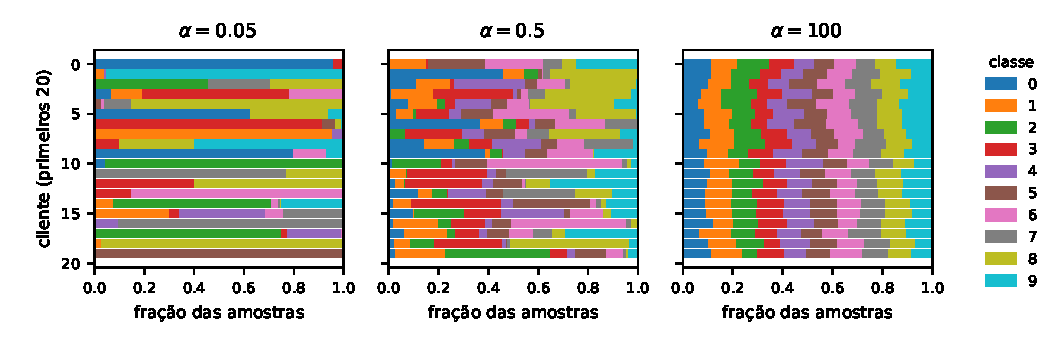
\includegraphics[width=0.92\textwidth]{figs/particoes.pdf}
    \caption{Distribuição de rótulos nos 20 primeiros dos 100 clientes para três valores de $\alpha$, em um conjunto balanceado de 10 classes com 5.000 amostras cada (como o CIFAR-10). Cada barra é um cliente, e as cores indicam a fração de cada classe. Gerada por \texttt{scripts/fig\_particoes.py} com semente 0 e mínimo de 5 amostras por cliente.}
    \label{fig:particoes}
\end{figure*}

Os algoritmos de referência (bloco B) entram em C1. Eles mostram se o ganho do FedProx, quando existe, é grande ou pequeno diante de alternativas que deslocam a correção para o servidor e não custam nada ao cliente.

\subsection{Fluxo de execução}
\label{sec:fluxo}

A Figura~\ref{fig:fluxo} resume o fluxo completo, da preparação dos dados à análise. Duas verificações antecedem a grade completa. A primeira é um \textbf{piloto} no Fashion-MNIST, com uma semente e 20 rodadas, que valida o \textit{pipeline} e mede o tempo real por execução para confirmar o orçamento. A segunda é o \textbf{teste de sanidade} entre FedProx com $\mu = 0$ e FedAvg: com a mesma semente e algoritmos determinísticos habilitados, as duas execuções devem produzir curvas de acurácia idênticas. Qualquer diferença indica falha no pareamento ou na implementação.

\begin{figure}[ht]
    \centering
    \begin{tikzpicture}[
        font=\scriptsize,
        etapa/.style={draw, rounded corners=2pt, fill=azul!6, text width=5.6cm, align=center, minimum height=0.55cm},
        dec/.style={draw, diamond, aspect=3.2, fill=gray!10, align=center, inner sep=1pt},
        arr/.style={-{Stealth[length=4pt]}, thick},
        node distance=0.3cm
    ]
        \node[etapa] (s1) {1. Preparar ambiente (Kaggle) e baixar datasets};
        \node[etapa, below=of s1] (s2) {2. Piloto: F-MNIST, 1 semente, 20 rodadas};
        \node[dec, below=of s2] (d1) {$\mu{=}0 \equiv$ FedAvg?\\ tempo ok?};
        \node[etapa, below=of d1] (s3) {3. Blocos A e B (exploratório, 5 sementes)};
        \node[etapa, below=of s3] (s4) {4. Escolher $\mu^*$ por dataset};
        \node[etapa, below=of s4] (s5) {5. Blocos C e D (tipos de desvio; 10 sementes novas)};
        \node[etapa, below=of s5] (s6) {6. Micro-experimento de custo em CPU (C4)};
        \node[etapa, below=of s6] (s7) {7. Análise: curvas, mapa $\alpha\times\mu$, Wilcoxon + Holm, TOST};
        \draw[arr] (s1) -- (s2);
        \draw[arr] (s2) -- (d1);
        \draw[arr] (d1) -- node[right]{sim} (s3);
        \draw[arr] (d1.east) -- ++(0.55,0) |- node[pos=0.25, right]{não: corrigir} (s2.east);
        \draw[arr] (s3) -- (s4);
        \draw[arr] (s4) -- (s5);
        \draw[arr] (s5) -- (s6);
        \draw[arr] (s6) -- (s7);
    \end{tikzpicture}
    \caption{Fluxo de execução experimental.}
    \label{fig:fluxo}
\end{figure}

Na etapa 7, o script de análise produz quatro artefatos: (i) curvas de acurácia por rodada, com média e desvio padrão entre sementes, para cada $\alpha$; (ii) um mapa de calor do ganho médio $\Delta$ do FedProx sobre o FedAvg, nos eixos $\alpha$ e $\mu$ (bloco A, descritivo); (iii) a tabela de $R_\tau$ e custo total até o alvo, com a fração de execuções que atinge $\tau$; e (iv) a tabela de testes estatísticos (Wilcoxon e TOST) dos blocos C e D. Esses artefatos são a base da Seção~\ref{sec:resultados}.

% \section{Resultados, Conclusões e Trabalhos Futuros}
\label{sec:resultados}

Esta seção sintetiza o que o trabalho produziu, delimita o alcance das conclusões e indica como ele pode ser continuado.

\subsection{Resultados experimentais}

\pendente{Esta subseção depende da execução dos blocos A--D e do micro-experimento. Substituir os marcadores pelos valores obtidos, inserir as figuras geradas por \texttt{analysis.py} (curvas de convergência por $\alpha$; mapa de calor $\alpha \times \mu$) e reescrever os parágrafos abaixo à luz dos dados.}

A Tabela~\ref{tab:resultados} apresenta, para o CIFAR-10, a acurácia final de FedAvg e FedProx com $\mu^*$ nas dez sementes confirmatórias, a diferença pareada com intervalo de confiança, o p-valor do Wilcoxon ajustado por Holm, o p-valor do teste de equivalência (TOST) e as rodadas até a acurácia-alvo. A mesma tabela para o Fashion-MNIST e os resultados dos algoritmos de referência ficam no repositório.

\begin{table}[ht]
    \centering\scriptsize
    \caption{FedAvg × FedProx ($\mu^* = $ \pendente{?}) no CIFAR-10, bloco D (10 sementes). Acurácia em \%, média $\pm$ desvio padrão.}
    \label{tab:resultados}
    \setlength{\tabcolsep}{3pt}
    \begin{tabular}{@{}lcccccc@{}}
        \toprule
        $\alpha$ & FedAvg & FedProx & $\Delta$ [IC 95\%] & $p_{\text{Holm}}$ & $p_{\text{TOST}}$ & $R_\tau$ (Avg/Prox) \\
        \midrule
        0,05 & \pendente{--} & \pendente{--} & \pendente{--} & \pendente{--} & \pendente{--} & \pendente{--} \\
        0,1  & \pendente{--} & \pendente{--} & \pendente{--} & \pendente{--} & \pendente{--} & \pendente{--} \\
        0,5  & \pendente{--} & \pendente{--} & \pendente{--} & \pendente{--} & \pendente{--} & \pendente{--} \\
        1    & \pendente{--} & \pendente{--} & \pendente{--} & \pendente{--} & \pendente{--} & \pendente{--} \\
        100  & \pendente{--} & \pendente{--} & \pendente{--} & \pendente{--} & \pendente{--} & \pendente{--} \\
        \bottomrule
    \end{tabular}
\end{table}

\textbf{QP1 (H1--H3).} \pendente{Descrever em que faixa de $\alpha$ o ganho do FedProx é significativo, se o melhor $\mu$ muda com $\alpha$ e se o ranking muda entre partição patológica e desvio de quantidade. Comparar com FedAvgM, FedAdam e SCAFFOLD.}

\textbf{QP2 (H4).} \pendente{Informar a razão entre as medianas do tempo por época (FedProx/FedAvg) na CPU de 1 thread, a diferença de memória de pico e o custo total até o alvo $C_\tau$ para cada $\alpha$.}

\subsection{Principais contribuições}

Em relação aos objetivos da Seção~\ref{sec:introducao}, o trabalho entrega:

\begin{itemize}[leftmargin=*, itemsep=2pt]
    \item \textbf{Levantamento sistemático focado em estudos comparativos (OE1).} São 22 estudos de 2021 a 2026, selecionados por critérios explícitos e reprodutíveis, com protocolo, tabelas por critério e planilha de triagem disponíveis no repositório. A análise mostrou que a literatura se contradiz sobre o FedProx e identificou três lacunas: $\mu$ não controlado, custo local não medido e ausência de um limiar de heterogeneidade.
    \item \textbf{Ambiente experimental reprodutível e de custo zero (OE2, OE3).} Inclui simulação com Flower e partições controladas, pareamento por semente e teste de sanidade $\mu = 0 \equiv$ FedAvg, tudo executável em GPUs gratuitas. O ambiente pode ser reaproveitado para avaliar outros algoritmos de agregação sem mudança no restante do \textit{pipeline}.
    \item \textbf{Evidência sobre quando o FedProx compensa (OE4--OE6).} \pendente{Resumir o mapa $\alpha \times \mu \times$ (acurácia, custo) obtido e a recomendação prática derivada, por exemplo: ``para $\alpha \leq$ X, usar FedProx com $\mu =$ Y; acima disso, FedAvg ou FedAvgM''.}
    \item \textbf{Medição isolada do custo do termo proximal em CPU restrita.} \pendente{Resumir o resultado do micro-experimento.} Nenhum dos estudos do levantamento relata essa medição no resumo.
\end{itemize}

\subsection{Limitações do trabalho}

\begin{itemize}[leftmargin=*, itemsep=2pt]
    \item \textbf{Simulação × implantação.} Todos os clientes rodam em uma única máquina, sem latência de rede, falhas de conexão nem diferenças reais de hardware. \citet{valli2026beyond} mostram que resultados de simulação podem divergir de implantações reais. O micro-experimento em CPU de um núcleo aproxima o custo de um dispositivo de borda, mas não o substitui.
    \item \textbf{Modelos e dados.} As CNNs são pequenas e os datasets são de imagens com dez classes balanceadas. Redes profundas, outros domínios (séries temporais, texto) ou desvio de atributos podem se comportar de outra forma. As conclusões valem para o regime estudado.
    \item \textbf{Hiperparâmetros fixos.} A taxa de aprendizado local e o número de épocas são os mesmos para todos os algoritmos e não foram otimizados para cada um. É uma escolha deliberada para isolar o efeito da agregação, mas pode favorecer algum algoritmo.
    \item \textbf{Grade de $\mu$ e orçamento.} Foram testados três valores de $\mu$, e os algoritmos de referência rodaram com apenas três sementes, por causa da cota gratuita de GPU.
    \item \textbf{Cobertura do levantamento.} Scopus e Web of Science não foram consultadas diretamente, e a triagem foi feita por título e resumo. Quatro estudos com resumo inacessível ficaram fora da análise.
\end{itemize}

\subsection{Possibilidades de continuidade}

As extensões mais diretas atacam as limitações acima:

\begin{itemize}[leftmargin=*, itemsep=2pt]
    \item \textbf{Validação em hardware real.} Executar FedAvg e FedProx com o mesmo código em um conjunto de Raspberry Pi ou celulares, usando o modo de implantação do Flower, e medir tempo, energia e tráfego de rede reais, como em \citet{carranco2025adhoc}.
    \item \textbf{Heterogeneidade de sistema.} Executar o cenário C5 (\textit{stragglers}), em que o FedProx aceita trabalho local parcial e onde, segundo \citet{cheng2026stragglers}, as diferenças entre os algoritmos são maiores.
    \item \textbf{$\mu$ adaptativo.} Se o melhor $\mu$ variar com $\alpha$, investigar regras que ajustem $\mu$ por rodada ou por cliente a partir de uma estimativa local da heterogeneidade.
    \item \textbf{Desvio de atributos e dados naturais.} Incluir o FEMNIST \citep{caldas2018leaf}, com heterogeneidade natural por escritor, e datasets de domínios de borda como sensores IoT e reconhecimento de atividades.
    \item \textbf{Mais algoritmos e modelos.} Estender a comparação a FedNova \citep{wang2020fednova} e a modelos maiores (ResNet), verificando se o custo relativo do termo proximal muda com o tamanho da rede.
\end{itemize}

\subsection{Aplicações futuras}

O resultado principal, um critério de escolha do algoritmo de agregação a partir do grau de heterogeneidade, é útil a quem projeta sistemas federados em borda. Alguns exemplos:

\begin{itemize}[leftmargin=*, itemsep=2pt]
    \item \textbf{Saúde conectada:} hospitais e dispositivos vestíveis com populações de pacientes muito diferentes, domínio mais frequente no levantamento \citep{mahmood2025alzheimer, mim2025healthcare}.
    \item \textbf{IoT industrial e cidades inteligentes:} sensores e câmeras fixos que observam fenômenos locais, como no reconhecimento de vagas \citep{bakr2026parkfl} e na previsão de geração renovável \citep{ghosh2026renewable}.
    \item \textbf{Enxames de drones e veículos:} clientes móveis com dados que mudam de distribuição conforme a missão \citep{hu2025uav}.
\end{itemize}

Em todos esses cenários, uma estimativa simples da heterogeneidade antes da implantação (por exemplo, a divergência entre as distribuições de rótulos dos clientes) pode ser cruzada com o mapa produzido aqui para decidir se o custo extra do FedProx nos dispositivos se justifica. O repositório aberto permite que essa avaliação seja refeita para o modelo e os dados de cada aplicação.

\subsection{Conclusão}

O trabalho partiu de uma constatação do levantamento bibliográfico: apesar de amplamente usado, o FedProx não tem uma vantagem consistente sobre o FedAvg na literatura recente, e os estudos raramente controlam $\mu$, o nível de heterogeneidade ou o custo no cliente. Para responder em quais condições o termo proximal compensa, foi desenhado um experimento pareado, reprodutível e de custo zero, que cruza tipo e nível de heterogeneidade com o valor de $\mu$ e mede tanto a qualidade do modelo quanto o custo local. \pendente{Concluir com a resposta às QP1 e QP2 em uma ou duas frases, com base nos resultados.}


\bibliographystyle{apalike2_ptBR}
\bibliography{referencias}

\end{document}
